\lecture{Лекция 6}{lec6}
\subtitle{Лекция 6 --- Алгебра логики. Часть 3 --- Примеры решения задач}

\frame[plain]
{\titlepage}	% Титульный слайд


\begin{frame}
\frametitle{Алгебра логики}

\begin{center}

\Huge
Задача 18 ЕГЭ
	
\end{center}


\end{frame}

\begin{frame}
\frametitle{Схема решения задачи 18}

Общая схема решения задач типа задачи 18 ЕГЭ: <<Найти число А для логического выражения>>
\begin{enumerate}
	\item Замена переменных для упрощения работы с выражением
	\item Приведение выражения к стандартному виду. Если требуется тождественная истинность, то дизъюнкция выражений, если тождественная ложность, то конъюнкция выражений.
	\item Определение <<проблемной ситуации>>: когда значение логического выражения зависит от А
	\item Формулирование условий и ограничений для числа А
	\item Поиск числа А
\end{enumerate}


\end{frame}

\begin{frame}[t]
\frametitle{Примеры задача 18}
\framesubtitle{Задачи с отрезками}

На числовой прямой даны отрезки $A = [70; 90]$, $B = [40; 60]$ и $C = [0; N]$ и функция \\
$F(x) = (\overline{(x \in A)} \rightarrow (x \in B) ) \wedge (\overline{(x \in C)} \rightarrow (x \in A) )$
При каком наименьшем числе $N$ функция $F(x)$ истинна более чем для $30$ целых чисел $x$?


	\only<1>{1. Введем обозначение $A=A(x)=x \in A$. Для В и С аналогично. 
	
	Получим $F(x) = (\overline{A} \rightarrow B ) \wedge (\overline{С} \rightarrow A )$}
	\only<2>{2. Преобразуем: 
	 $$F(x) = \underbrace{(\overline{A} \rightarrow B )}_{A \vee B} \wedge \underbrace{(\overline{С} \rightarrow A )}_{C \vee A}=(A \vee B) \wedge (C \vee A)$$
	 $$F(x) = \underbrace{(A\wedge C) \vee \underbrace{(A\wedge A)}_{A}}_{Поглощение A} \vee (B \wedge C) \vee \underbrace{(B\wedge A)}_{Поглощение A}=A \vee (B\wedge C)
	$$}
	
\end{frame}

\begin{frame}[t]
\frametitle{Примеры задача 18}
\framesubtitle{Задачи с отрезками}

	
	3. нарисуем отрезки на числовой оси:\\
	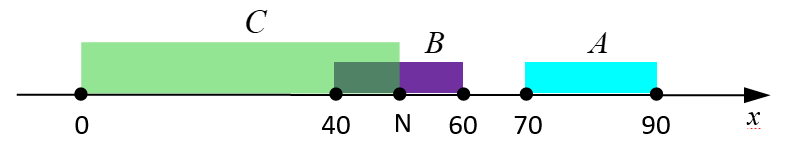
\includegraphics[height=2cm]{images/t18_1}
	\pause
	Составим таблицу для всех частей числовой прямой.
	\begin{tabular}{|c|c|c|c|c|}
\hline 
Интервал & A & B & C & F\tabularnewline
\hline 
$(-\infty;0]$ & 0 & 0 &  & 0\tabularnewline
\hline 
$[0;40]$ & 0 & 0 &  & 0\tabularnewline
\hline 
$[40;60]$ & 0 & 1 &  & \tabularnewline
\hline 
$[60;70]$ & 0 & 0 &  & 0\tabularnewline
\hline 
$[70;90]$ & 1 & 0 &  & 1\tabularnewline
\hline 
$[90;+\infty)$ & 0 & 0 &  & 0\tabularnewline
\hline 
\end{tabular}

	
	


\end{frame}

\begin{frame}[t]
\frametitle{Примеры задача 18}
\framesubtitle{Задачи с отрезками}

	
	Определим <<ПРОБЛЕМУ>>: когда нужен отрезок $C$?
	\begin{tabular}{|c|c|c|c|c|}
\hline 
Интервал & A & B & C & F\tabularnewline
\hline 
$(-\infty;0]$ & 0 & 0 & не влияет & 0\tabularnewline
\hline 
$[0;40]$ & 0 & 0 & не влияет & 0\tabularnewline
\hline 
$[40;60]$ & 0 & 1 & \textbf{ПРОБЛЕМА} & \tabularnewline
\hline 
$[60;70]$ & 0 & 0 & не влияет & 0\tabularnewline
\hline 
$[70;90]$ & 1 & 0 & не влияет & 1\tabularnewline
\hline 
$[90;+\infty)$ & 0 & 0 & не влияет & 0\tabularnewline
\hline 
\end{tabular}

	\pause
	
	4. Получается, что всегда есть $90-70+1=21$ число для которого выражение истинно.\\
	Нам нужно набрать более 30 чисел. Значит число $N$ должно попасть в отрезок $[40;60]$
	
	\pause 
	5. Следовательно:  $10=N-40+1 \Rightarrow N=49$
	


\end{frame}

\begin{frame}[t]
\frametitle{Примеры задача 18}
\framesubtitle{Задачи с серией условий}

Для какого наибольшего целого числа А формула
$$( (x \leq 9) \rightarrow (x\cdot x \leq A) ) \wedge ( (y\cdot y \leq A) \rightarrow (y \leq 9) )$$
тождественно истинна (то есть принимает значение 1 при любых целых неотрицательных значениях переменных x и y)?
	\begin{enumerate}
		\item Замена не требуется 	\pause 
		\item Преобразование не требуется 	\pause 
		\item Когда возникает <<ПРОБЛЕМА>>?  	\pause 
		$$( \underbrace{(x \leq 9)}_{1} \rightarrow (x\cdot x \leq A) ) \wedge ( (y\cdot y \leq A) \rightarrow \underbrace{(y \leq 9)}_{0} )$$ В этом случае все зависит от А.
		
		
	\end{enumerate}
	
	
	
\end{frame}

\begin{frame}[t]
\frametitle{Примеры задача 18}
\framesubtitle{Задачи с серией условий}

Для какого наибольшего целого числа А формула
$$( (x \leq 9) \rightarrow (x\cdot x \leq A) ) \wedge ( (y\cdot y \leq A) \rightarrow (y \leq 9) )$$
тождественно истинна (то есть принимает значение 1 при любых целых неотрицательных значениях переменных x и y)?
	\begin{enumerate}
		\setcounter{enumi}{3}
		\item $x \leq 9=1 \Rightarrow x=\{9,8,7, \ldots\}$\\ 	\pause 
		      значит $(x^2 \leq A)=1 \Rightarrow A=\{81,82,83, \ldots\}$\\ 	\pause 
		      $y \leq 9=0 \Rightarrow y>9 \Rightarrow y=\{10,11,12,\ldots\}$\\  	\pause 
					значит $(y^2 \leq A)=0 \Rightarrow y^2>A \Rightarrow A=\{99,98,97, \ldots\}$\\ 	\pause 
					следовательно $81\leq A \leq 99$ 	\pause 
	 \item наименьшее $A=81$, наибольшее $A=99$.
		
	\end{enumerate}
	
	
	
\end{frame}

\begin{frame}[t]
\frametitle{Примеры задача 18}
\framesubtitle{Задачи с серией условий}

Укажите наименьшее целое значение А, при котором выражение
$$(y + 2x < A) \vee (3y + 2x > 120) \vee (3y - x > 30)$$
истинно для любых целых положительных значений x и y.

	\begin{enumerate}
		\item Замена не требуется 	\pause 
		\item Преобразование не требуется 	\pause 
		\item Когда возникает <<ПРОБЛЕМА>>? 	\pause 
		$$(y + 2x < A) \vee \underbrace{(3y + 2x > 120)}_{0} \vee \underbrace{(3y - x > 30)}_{0}$$
		В этом случае все зависит от А.
		
		
	\end{enumerate}
	
	
\end{frame}

\begin{frame}[t]
\frametitle{Примеры задача 18}
\framesubtitle{Задачи с серией условий}
\begin{enumerate}
		\setcounter{enumi}{3}
		\item $(3y + 2x > 120)=0 \Rightarrow 3y + 2x \leq 120 (1)$\\  	\pause 
		      $(3y - x > 30)=0 \Rightarrow 3y - x \leq 30 (2)$\\ 
					умножим второе неравенство на 2 и сложим с первым \\
					$3y+2x+6y-2x \leq 120+60$\\
					$9y \leq 180 \Rightarrow 0 < y \leq 20 $\\
					В этом случае должно быть $(y + 2x < A)=1, y < A-2x (3)$\\ 	\pause 
					Следовательно нам нужно найти наибольшее возможное x и выбрать $A$ так чтобы $A-2x$ было положительным неравенство (3) выполнялось для всех $y$\\ 	\pause 
					Из (1) Наибольший $x$ соответствует наименьшему возможному $y=1$\\
					$3+2x\leq 120 \Rightarrow x \leq 58 \Rightarrow \underbrace{1+2\cdot 58}_{117} < A \Rightarrow A \geq 118$\\ 	\pause 
	 \item наименьшее $A=118$.
		
	\end{enumerate}
	
	
	
\end{frame}

\begin{frame}[t]
\frametitle{Примеры задача 18}
\framesubtitle{Задачи с поразрядными операциями}

Применение логической операции <<поразрядно>> к числам $x$ и $y$ $x R y$, $R=\{\vee, \wedge, \rightarrow, \oplus, \equiv \}$:
\begin{enumerate}
	\item Перевести оба числа в двоичную систему счисления 	\pause 
	\item Применить операцию $R$ к каждой паре разрядов. (считаем, что слева от первого значащаего разряда стоят нули, например $1010=0001010$
\end{enumerate}
	
\end{frame}

\begin{frame}[t]
\frametitle{Примеры задача 18}
\framesubtitle{Задачи с поразрядными операциями}
Пример. $x=52, y=21$, $52=110100_2,21=10101_2$
\only<1>{
$$52 \wedge 21 = 20$$
\begin{tabular}{ccccccc}
\multirow{2}{*}{$\wedge$} & 1 & 1 & 0 & 1 & 0 & 0\tabularnewline
 & 0 & 1 & 0 & 1 & 0 & 1\tabularnewline
\cline{2-7} \cline{3-7} \cline{4-7} \cline{5-7} \cline{6-7} \cline{7-7} 
 & 0 & 1 & 0 & 1 & 0 & 0\tabularnewline
\end{tabular}
}
\only<2>{
$$52 \vee 21 = 53$$
\begin{tabular}{ccccccc}
\multirow{2}{*}{$\vee$}
 & 1 & 1 & 0 & 1 & 0 & 0\tabularnewline
 & 0 & 1 & 0 & 1 & 0 & 1\tabularnewline
\cline{2-7} \cline{3-7} \cline{4-7} \cline{5-7} \cline{6-7} \cline{7-7} 
 & 1 & 1 & 0 & 1 & 0 & 1\tabularnewline
\end{tabular}
}
\only<3>{
$$52 \rightarrow 21 = 31$$
\begin{tabular}{ccccccc}
\multirow{2}{*}{$\rightarrow$}
 & 1 & 1 & 0 & 1 & 0 & 0\tabularnewline
 & 0 & 1 & 0 & 1 & 0 & 1\tabularnewline
\cline{2-7} \cline{3-7} \cline{4-7} \cline{5-7} \cline{6-7} \cline{7-7} 
 & 0 & 1 & 1 & 1 & 1 & 1\tabularnewline
\end{tabular}
}	
\only<4>{
$$52 \equiv 21 = 30$$
\begin{tabular}{ccccccc}
\multirow{2}{*}{$\equiv$}
 & 1 & 1 & 0 & 1 & 0 & 0\tabularnewline
 & 0 & 1 & 0 & 1 & 0 & 1\tabularnewline
\cline{2-7} \cline{3-7} \cline{4-7} \cline{5-7} \cline{6-7} \cline{7-7} 
 & 0 & 1 & 1 & 1 & 1 & 0\tabularnewline
\end{tabular}
}
\only<5>{
$$52 \oplus 21 = 33$$
\begin{tabular}{ccccccc}
\multirow{2}{*}{$\oplus$}
 & 1 & 1 & 0 & 1 & 0 & 0\tabularnewline
 & 0 & 1 & 0 & 1 & 0 & 1\tabularnewline
\cline{2-7} \cline{3-7} \cline{4-7} \cline{5-7} \cline{6-7} \cline{7-7} 
 & 1 & 0 & 0 & 0 & 0 & 1\tabularnewline
\end{tabular}
}

	
	
	
\end{frame}


\begin{frame}[t]
\frametitle{Примеры задача 18}
\framesubtitle{Задачи с поразрядными операциями 1}

Введём выражение $M \& K$, обозначающее поразрядную конъюнкцию M и K. Определите наименьшее натуральное число $A$, такое что выражение
$$( x \& 49 \neq 0) \rightarrow ((x \& 33 = 0) \rightarrow (x \& A \neq 0))$$
тождественно истинно (то есть принимает значение 1 при любом натуральном значении переменной x)?

	\begin{enumerate}
		\item Замена: $Z_{n}=Z(n,x)=\begin{cases}
0 & x\&n\neq0\\
1 & x\&n=0
\end{cases}$ \\ 	\pause 
получим $\overline{Z_{49}} \rightarrow (Z_{33} \rightarrow \overline{Z_A})$
		\item Преобразование к стандартному виду: 
		$Z_{49} \vee \overline{Z_{33}} \vee \overline{Z_A}$ 	\pause 
		\item Когда возникает <<ПРОБЛЕМА>>?  	
		      $Z_{49}=0$ и $Z_{33}=1$ \\Теперь все зависит от $A$!
					
	\end{enumerate}
	
	
\end{frame}

\begin{frame}[t]
\frametitle{Примеры задача 18}
\framesubtitle{Задачи с поразрядными операциями 1}

	\begin{enumerate}
	\setcounter{enumi}{3}
		\item Введем обозначения:\\
		$*=\{0,1\}$ --- любая цифра\\ 	\pause 
		$b=\{0,1\}$ --- тоже любая цифра, но если есть несколько $b$, то они все не могут быть равны $0$.\\ 	\pause 
		$a=\{0,1\}$ --- тоже любая цифра, но если есть несколько $a$, то они все не могут быть равны $1$.\\ 
					
	\end{enumerate}
	
	
\end{frame}


\begin{frame}[t]
\frametitle{Примеры задача 18}
\framesubtitle{Задачи с поразрядными операциями 1}

	\begin{enumerate}
	\setcounter{enumi}{3}
		\item 
		Переведем 49 и 33 в двоичную систему счисления.\\ 
		$49=110001_2$,$33=100001_2$\\
		\textcolor[rgb]{1,1,1}{ddd}\\ 	\pause 
		Какие числа делают так, что $Z_{49}=0$? Те, которые при побитовой конъюнкции со 49 не формируют 0\\
		шаблон плохого числа для 49: \texttt{bb***b}\\
		\textcolor[rgb]{1,1,1}{ddd}\\ 	\pause 
		Какие числа делают так, что $Z_{33}=1$? Те, которые при побитовой конъюнкции с 33 формируют 0\\
		шаблон плохого числа для 33: \texttt{0****0}
		
							
	\end{enumerate}
	
	
\end{frame}


\begin{frame}[t]
\frametitle{Примеры задача 18}
\framesubtitle{Задачи с поразрядными операциями 1}

	\begin{enumerate}
	\setcounter{enumi}{3}
		\item 
				
		Нужно построить общий шаблон плохого числа и для 49 и для 33\\ 	\pause 
		\begin{tabular}{ccccccc}
\multirow{2}{*}{$\wedge$}
 & b & b & * & * & * & b\tabularnewline
 & 0 & * & * & * & * & 0\tabularnewline
\cline{2-7} \cline{3-7} \cline{4-7} \cline{5-7} \cline{6-7} \cline{7-7} 
 & 0 & b & * & * & * & 0\tabularnewline
\end{tabular}
		
		
		\item Что должно сделать А? Первые два выражения равны 0, значит $\overline{Z_A}=1$ или
		$Z_A=0$.\\ 	\pause 
		Наименьшее A, которое при побитовой конъюнкции с x=\texttt{0b***0} не формирует 0 равно: $A=10000_2=16$.
					
	\end{enumerate}
	
	
\end{frame}

\begin{frame}[t]
\frametitle{Примеры задача 18}
\framesubtitle{Задачи с поразрядными операциями 2}

Введём выражение M \& K, обозначающее поразрядную конъюнкцию M и K. Определите наименьшее натуральное число $A$, такое что выражение
$$( (x \& 28 \neq 0) \vee  (x \& 45 \neq 0)) \rightarrow ((x \& 48 = 0) \rightarrow (x \& A \neq 0))$$
тождественно истинно (то есть принимает значение 1 при любом натуральном значении переменной x)?

	\begin{enumerate}
		\item Замена: $Z_{n}=Z(n,x)=\begin{cases}
0 & x\&n\neq0\\
1 & x\&n=0
\end{cases}$ \\
получим $(\overline{Z_{28}}\vee \overline{Z_{45}}) \rightarrow (Z_{48} \rightarrow \overline{Z_A})$ 	\pause 
		\item Преобразование к стандартному виду: 
		$Z_{28} \wedge Z_{45}  \vee \overline{Z_{48}} \vee \overline{Z_A}$ 	\pause 
		\item Когда возникает <<ПРОБЛЕМА>>? 
		      $Z_{28} \wedge Z_{45}=0$ и $Z_{48}=1$ \\Теперь все зависит от $A$!
					
	\end{enumerate}
	
	
\end{frame}


\begin{frame}[t]
\frametitle{Примеры задача 18}
\framesubtitle{Задачи с поразрядными операциями 2}

	\begin{enumerate}
	\setcounter{enumi}{3}
		\item 
		Переведем 48,45 и 28 в двоичную систему счисления.\\
		$48=110000_2$, $45=101101_2$, $28=11100_2$\\
		\textcolor[rgb]{1,1,1}{ddd}\\ 	\pause 
		Какие числа делают так, что $Z_{28} \wedge Z_{45}=0$? Те, которые при побитовой конъюнкции с 45 или 28 не формируют 0\\
		шаблон плохого числа для 45: \texttt{b*bb*b}\\
		шаблон плохого числа для 28: \texttt{ bbb**}\\ 	\pause 
		Общее плохое число: \texttt{bbbb*b}\\  
		\textcolor[rgb]{1,1,1}{ddd}\\ 	\pause 
		Какие числа делают так, что $Z_{48}=1$? Те, которые при побитовой конъюнкции с 48 формируют 0\\ 	\pause 
		шаблон плохого числа для 48: \texttt{00****}
		
							
	\end{enumerate}
	
	
\end{frame}


\begin{frame}[t]
\frametitle{Примеры задача 18}
\framesubtitle{Задачи с поразрядными операциями 2}

	\begin{enumerate}
	\setcounter{enumi}{3}
		\item 
				
		Нужно построить общий шаблон плохого числа и для 28, 45 и для 48\\ 	\pause 
		\begin{tabular}{ccccccc}
\multirow{2}{*}{$\wedge$}
 & b & b & b & b & * & b\tabularnewline
 & 0 & 0 & * & * & * & *\tabularnewline
\cline{2-7} \cline{3-7} \cline{4-7} \cline{5-7} \cline{6-7} \cline{7-7} 
 & 0 & 0 & b & b & * & b\tabularnewline
\end{tabular}
		
		
		\item Что должно сделать А? Первые два выражения равны 0, значит $\overline{Z_A}=1$ или
		$Z_A=0$.\\ 	\pause 
		Наименьшее A, которое при побитовой конъюнкции с x=\texttt{00bb*b} не формирует 0 равно: $A=1101_2=13$.
					
	\end{enumerate}
	
	
\end{frame}



\begin{frame}[t]
\frametitle{Примеры задача 18}
\framesubtitle{Задачи с поразрядными операциями 3}

Определите наибольшее натуральное число A, при котором выражение
$$((x \& A \neq 0) \rightarrow (x \& 39 = 7)) \vee (x \& 30 \neq 6)$$
тождественно истинно (то есть принимает значение 1 при любом натуральном значении переменной x)?

	\begin{enumerate}
		\item Замена:  $(\overline{Z_{A}}\rightarrow Z_{39}) \vee  \overline{Z_30})$ 	\pause 
		\item Преобразование к стандартному виду: 
		$Z_{A} \vee Z_{39} \vee \overline{Z_{30}}$ 	\pause 
		\item Когда возникает <<ПРОБЛЕМА>>? 
		      $Z_{30}=1$ и $Z_{39}=0$ \\Теперь все зависит от $A$!
					
	\end{enumerate}
	
	
\end{frame}


\begin{frame}[t]
\frametitle{Примеры задача 18}
\framesubtitle{Задачи с поразрядными операциями 3}

	\begin{enumerate}
	\setcounter{enumi}{3}
		\item 
		Переведем 30 и 39 в двоичную систему счисления.\\ 	\pause 
		$30=11110_2$, $39=100111_2$
		\textcolor[rgb]{1,1,1}{ddd}\\ 	\pause 
		Какие числа делают так, что $Z_{30} =1$? Те, которые при побитовой конъюнкции с 30 формируют 6\\
		шаблон плохого числа для 30: \texttt{**11*}\\
		\textcolor[rgb]{1,1,1}{ddd}\\ 	\pause 
		Какие числа делают так, что $Z_{39}=0$? Те, которые при побитовой конъюнкции с 39 НЕ формируют 7\\
		шаблон плохого числа для 39: \texttt{0**aaa} или \texttt{1*****}\\
		\textcolor[rgb]{1,1,1}{ddd}\\ 	\pause 
		т.е. либо есть 0 в последних трех битах, либо первый бит равен 1.
		
							
	\end{enumerate}
	
	
\end{frame}


\begin{frame}[t]
\frametitle{Примеры задача 18}
\framesubtitle{Задачи с поразрядными операциями 3}

	\begin{enumerate}
	\setcounter{enumi}{3}
		\item
		Нужно построить общий шаблон плохого числа и для 30 и 39\\ 	\pause 
		\begin{tabular}{ccccccc}
\multirow{2}{*}{$\wedge$}
 & * & * & * & 1 & 1 & * \tabularnewline
 & 0 & * & * & a & a & a  \tabularnewline
 & 1 & * & * & * & * & *  \tabularnewline
\cline{2-7} \cline{3-7} \cline{4-7} \cline{5-7} \cline{6-7} \cline{7-7} 
 & 0 & * & * & 1 & 1 & 0 \tabularnewline
 & 1 & * & * & 1 & 1 & * \tabularnewline
\end{tabular}
		
		
		\item Что должно сделать А? 	\pause  Первые два выражения равны 0, значит $Z_A=1$.\\ 	\pause 
		Наибольшее A, которое при побитовой конъюнкции с x=\texttt{0**110} или x=\texttt{1**11*} формирует 0 равно: $A=11000_2=24$.
					
	\end{enumerate}
	
	
\end{frame}

\begin{frame}[t]
\frametitle{Примеры задача 18}
\framesubtitle{Задачи с делимостью}

Обозначим через $ДЕЛ(n, m)$ утверждение <<натуральное число n делится без остатка на натуральное число m>>. Для какого наименьшего натурального числа А формула
$$ДЕЛ(x, А) \rightarrow (\neg ДЕЛ(x, 21) + ДЕЛ(x, 35))$$
тождественно истинна (то есть принимает значение 1 при любом натуральном значении переменной х)? 

	\begin{enumerate}
		\item Замена: $Z_{n}=Z(n,x)=\begin{cases}
0 & x\;mod\;n\neq 0\\
1 & x\;mod\;n=0
\end{cases}$ \\
получим $(Z_{A} \rightarrow (\overline{Z_{21}} \vee Z_{35})$ 	\pause 
		\item Преобразование к стандартному виду: 
		$Z_{35} \vee \overline{Z_{21}} \vee \overline{Z_A}$ 	\pause 
		\item Когда возникает <<ПРОБЛЕМА>>? 
		      $Z_{35} =0$ и $Z_{21}=1$ \\Теперь все зависит от $A$!				
	\end{enumerate}	
\end{frame}


\begin{frame}[t]
\frametitle{Примеры задача 18}
\framesubtitle{Задачи с делимостью}
	\begin{enumerate}
	\setcounter{enumi}{3}
		\item 
		Какие числа делают так, что $Z_{35} =0$? Те, которые не делятся на 35\\
		шаблон плохого числа для 35: $x=35n+r, r \neq 0$\\ 	\pause 
		
		\textcolor[rgb]{1,1,1}{ddd}\\
		Какие числа делают так, что $Z_{21}=1$? Те, которые делятся на 21 без остатка\\
		шаблон плохого числа для 21: $x=21m$
								
	\end{enumerate}
	
	
\end{frame}


\begin{frame}[t]
\frametitle{Примеры задача 18}
\framesubtitle{Задачи с поразрядными операциями 2}

	\begin{enumerate}
	\setcounter{enumi}{3}
		\item 
				
		Нужно построить общий шаблон плохого числа и для 21 и 35\\
		т.е. число делится на $21=3\cdot 7$ и не делится на $35=5\cdot 7$\\ 	\pause 
		$$ 
		x=21,42,63,\ldots,\cancel{105},126,\ldots,\cancel{210},231,\ldots
		$$ 	\pause 
	  Пусть $A=n$. Рассмотрим $x=21n$ Тогда $x$ делится на 21 и делится на n.\\
		Следовательно мы должны выбрать $n$, такое что $21n$ делится на 35.
		\pause 
		\item Что должно сделать А? Первые два выражения равны 0, значит $\overline{Z_A}=1$ или
		$Z_A=0$.\\ 	\pause 
		Наименьшее A, для которого $21n$ делится на 35 $A=5$.
					
	\end{enumerate}
	
	
\end{frame}


\begin{frame}
\frametitle{Алгебра логики}

\begin{center}

\Huge
Задача 23 ЕГЭ\\
Системы логических уравнений
	
\end{center}


\end{frame}

\begin{frame}[t]
\frametitle{Примеры задача 23}
\framesubtitle{Дерево решений (метод отображений)}
Сколько различных решений имеет система логических уравнений 
\begin{align*}
(x_1 \rightarrow (x_2 \wedge y_2)) \wedge (y_1 \rightarrow y_2) = 1\\
(x_2 \rightarrow (x_3 \wedge y_3)) \wedge (y_2 \rightarrow y_3) = 1\\
\ldots \\
(x_7 \rightarrow (x_8 \wedge y_8)) \wedge (y_7 \rightarrow y_8) = 1
\end{align*}


где $x_1, \ldots, x_8, y_1, \ldots, y_8$, --- логические переменные. В ответе не нужно перечислять все различные наборы значений переменных, при которых выполнено данное равенство. В качестве ответа нужно указать количество таких наборов.

	
\end{frame}

\begin{frame}[t]
\frametitle{Примеры задача 23}
\framesubtitle{Дерево решений  (метод отображений)}

\begin{block}{Решение}
Если мы посмотрим на уравнения, то увидим, что в первом есть пара $(x_1,y_1)$ и $(x_2,y_2)$. А во втором
$(x_2,y_2)$ и $(x_3,y_3)$. Тогда решения системы можно выписать в виде дерева.

\begin{enumerate}
	\item Выписываем возможные наборы значений для пары $(x_1,y_1)$ и находим допустимые наборы значений для пары $(x_2,y_2)$ \\ 	\pause 
\begin{tabular}{|c|c|c|c|c|}
\hline 
x1y1 & 00 & 01 & 10 & 11\tabularnewline
\hline 
\hline 
x2y2 & \textbf{00,01,10,11} & \textbf{01,11} & \textbf{11} & \textbf{11}\tabularnewline
\hline 
\end{tabular} 	\pause 
\item Далее расчет делаем в таблице\\
\begin{tabular}{|c|c|c|c|c|c|c|c|c|}
\hline 
 & x1y1 & x2y2 & x3y3 & x4y4 & x5y5 & x6y6 & x7y7 & x8y8\tabularnewline
\hline 
00 & 1 & 1 & 1 & 1 & 1 & 1 & 1 & 1\tabularnewline
\hline 
01 & 1 & 2 & 3 & 4 & 5 & 6 & 7 & 8\tabularnewline
\hline 
10 & 1 & 1 & 1 & 1 & 1 & 1 & 1 & 1\tabularnewline
\hline 
11 & 1 & 4 & 8 & 13 & 19 & 26 & 34 & 43\tabularnewline
\hline 
\end{tabular} 	\pause 
\item Ответ 1+8+1+43=53
\end{enumerate}




\end{block}
	
\end{frame}

\begin{frame}[t]
\frametitle{Примеры задача 23}
\framesubtitle{Дерево решений  (метод отображений)}

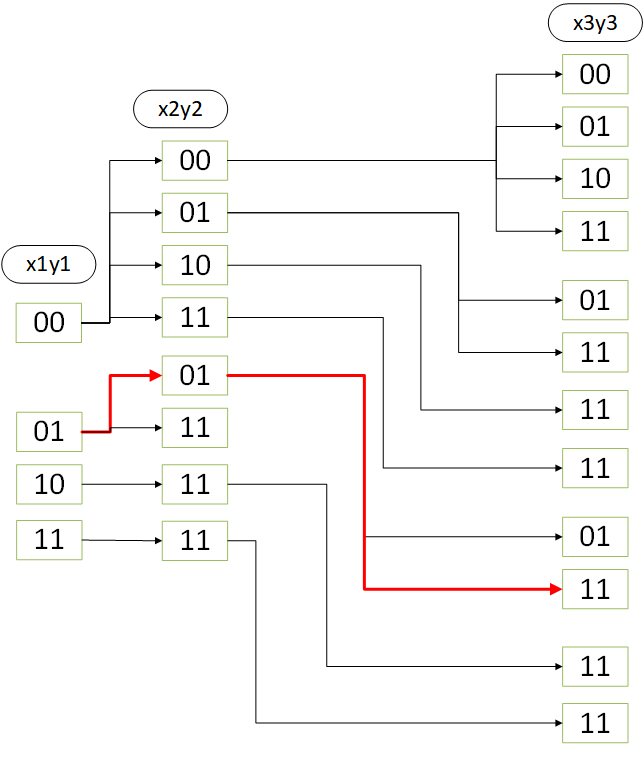
\includegraphics[height=7cm]{images/t23_1}\\
	
\end{frame}




\begin{frame}[t]
\frametitle{Примеры задача 23}
\framesubtitle{Дерево решений 2 (метод отображений)}
Сколько различных решений имеет система логических уравнений 
\begin{align*}
(X1 \wedge X2) \vee (\neg X1 \wedge \neg X2) \vee (X2 \wedge X3) \vee (\neg X2 \wedge \neg X3) = 1\\
(X2 \wedge X3) \vee (\neg X2 \wedge \neg X3) \vee (X3 \wedge X4) \vee (\neg X3 \wedge \neg X4) = 1\\
\ldots\\
(X8 \wedge X9) \vee (\neg X8 \wedge \neg X9) \vee (X9 \wedge X10) \vee (\neg X9 \wedge \neg X10) = 1\\
\end{align*}


где $x_1, \ldots, x_{10}$, --- логические переменные. В ответе не нужно перечислять все различные наборы значений переменных, при которых выполнено данное равенство. В качестве ответа нужно указать количество таких наборов.

	
\end{frame}

\begin{frame}[t]
\frametitle{Примеры задача 23}
\framesubtitle{Дерево решений 2 (метод отображений)}

\begin{block}{Решение}
Если мы посмотрим на уравнения, то увидим, что в первом есть пара $(x_1,x_2)$ и $(x_2,x_3)$. А во втором
$(x_2,x_3)$ и $(x_3,x_4)$. 
	\pause 

Если мы рассмотрим пару строк, то получим, что пара $(x_1,x_2)$ переходит в пару $(x_3,x_4)$, если рассмотреть две строки. Тогда решения системы можно выписать в виде дерева.

\end{block}
	
\end{frame}

\begin{frame}[t]
\frametitle{Примеры задача 23}
\framesubtitle{Дерево решений 2 (метод отображений)}

\begin{block}{Решение}
\begin{enumerate}
	\item Выписываем возможные наборы значений для пары $(x_1,x_2)$ и находим допустимые наборы значений для пары $(x_3,x_4)$ \\ 	\pause 
\begin{tabular}{|c|c|c|c|c|}
\hline 
x1x2 & 00 & 01 & 10 & 11\tabularnewline
\hline 
\hline 
x3x4 & \textbf{00,01,11} & \textbf{10,11} & \textbf{00,01} & \textbf{00,10,11}\tabularnewline
\hline 
\end{tabular} 	\pause 
\item Далее расчет делаем в таблице\\
\begin{tabular}{|c|c|c|c|c|c|}
\hline 
 & x1x2 & x3x4 & x5x6 & x7x8 & x9x10 \tabularnewline
\hline 
00 & 1 & 3 & 8 & 21 & 55 \tabularnewline
\hline 
01 & 1 & 2 & 5 & 13 & 34 \tabularnewline
\hline 
10 & 1 & 2 & 5 & 13 & 34 \tabularnewline
\hline 
11 & 1 & 3 & 8 & 21 & 55 \tabularnewline
\hline 
\end{tabular}
\item Ответ 55+34+34+55=178
\end{enumerate}
\end{block}
	
\end{frame}


\begin{frame}[t]
\frametitle{Примеры задача 23}
\framesubtitle{Дерево решений 3 (метод отображений)}
Сколько различных решений имеет система логических уравнений 
\begin{align*}
\neg(x1 \equiv x2) \wedge \neg(x1 \equiv x3) \wedge (x2 \equiv x3) = 0\\
\neg(x3 \equiv x4) \wedge \neg(x3 \equiv x5) \wedge (x4 \equiv x5) = 0\\
\neg(x5 \equiv x6) \wedge \neg(x5 \equiv x7) \wedge (x6 \equiv x7) = 0\\
\neg(x7 \equiv x8) \wedge \neg(x7 \equiv x9) \wedge (x8 \equiv x9) = 0
\end{align*}

где $x_1, \ldots, x_{9}$, --- логические переменные. В ответе не нужно перечислять все различные наборы значений переменных, при которых выполнено данное равенство. В качестве ответа нужно указать количество таких наборов.
	
\end{frame}

\begin{frame}[t]
\frametitle{Примеры задача 23}
\framesubtitle{Дерево решений 3 (метод отображений)}
\setlength{\columnsep}{0.4cm}
\begin{multicols}{3}
[
\textbf{Решение}\\
1.	для построения отображения построим таблицу решения первого уравнения
]
 
\begin{tabular}{|c|c|c|}
\hline 
x1 & x2 & x3\tabularnewline
\hline 
\multirow{4}{*}{0} & \multirow{2}{*}{0} & 0\tabularnewline
\cline{3-3} 
 &  & 1\tabularnewline
\cline{2-3} \cline{3-3} 
 & \multirow{2}{*}{1} & 0\tabularnewline
\cline{3-3} 
 &  & \tabularnewline
\hline 
\multirow{4}{*}{1} & \multirow{2}{*}{0} & \tabularnewline
\cline{3-3} 
 &  & 1\tabularnewline
\cline{2-3} \cline{3-3} 
 & \multirow{2}{*}{1} & 0\tabularnewline
\cline{3-3} 
 &  & 1\tabularnewline
\hline 
\end{tabular}
 
\columnbreak
 
Обратим внимание, что первое и второе уравнение связаны через переменные $x_1, x_3$. \\Построим отображение $x_1 \rightarrow x_3$.
\columnbreak
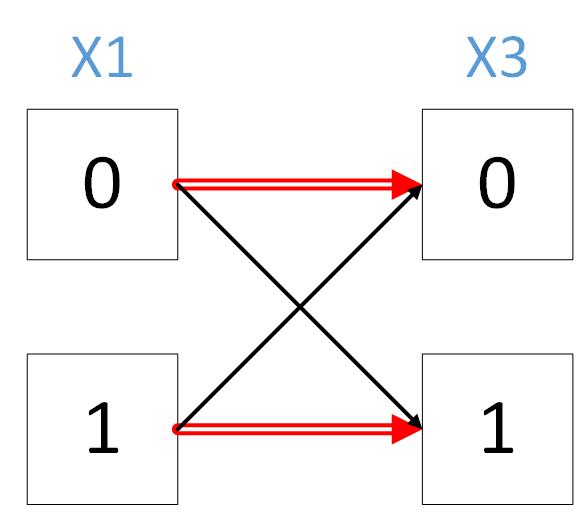
\includegraphics[height=3cm]{images/t23_2}
\end{multicols}
	
\end{frame}


\begin{frame}[t]
\frametitle{Примеры задача 23}
\framesubtitle{Дерево решений 3 (метод отображений)}
2.	В таблицу необходимо включить переменные $x_1,x_3,x_5, x_7 и x_9$ 

\begin{tabular}{|c|c|c|c|c|c|}
\hline
 & $x_1$ & $x_3$ & $x_5$ & $x_7$ &  $x_9$ \tabularnewline
\hline
0 & 1 & 3 & 9 & 27 &  81 \tabularnewline
1 & 1 & 3 & 9 & 27 &  81 \tabularnewline
\hline
\end{tabular}
	
3. складываем все результаты: 81 + 81 = 162.

	
\end{frame}

\begin{frame}[t]
\frametitle{Примеры задача 23}
\framesubtitle{Дерево решений 4 (метод отображений)}
Сколько различных решений имеет система логических уравнений 
\begin{align*}
(x1 \wedge x2) \vee (x1 \vee x3) \wedge (x1 \vee y1)=0\\
(x2 \wedge x3) \vee (x2 \vee x4) \wedge (x2 \vee y2)=1\\
(x3 \wedge x4) \vee (x3 \vee x5) \wedge (x3 \vee y3)=0\\
(x4 \wedge x5) \vee (x4 \vee x6) \wedge (x4 \vee y4)=1\\
(x5 \wedge x6) \vee (x5 \vee x7) \wedge (x5 \vee y5)=0\\
(x6 \wedge x7) \vee (x6 \vee x8)  \wedge (x6 \vee y6)=1
\end{align*}

где $x_1, \ldots, x_{9}$, --- логические переменные. В ответе не нужно перечислять все различные наборы значений переменных, при которых выполнено данное равенство. В качестве ответа нужно указать количество таких наборов.
	
\end{frame}

\begin{frame}[t]
\frametitle{Примеры задача 23}
\framesubtitle{Дерево решений 4 (метод отображений)}

\textbf{Решение}\\
1.	Для построения отображения построим таблицу решения первого уравнения 
Обратим внимание, что первое и второе уравнение связаны через переменные $x_2, x_3$. \\
Необходимо построить отображение $(x_1;x_2)$ на $(x_2;x_3)$ \\и $(x_2;x_3)$ на $(x_3;x_4)$\\
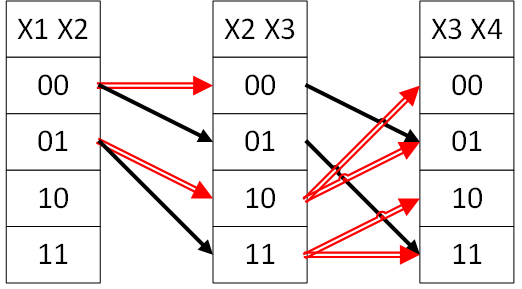
\includegraphics[height=4cm]{images/t23_3}


	
\end{frame}

\begin{frame}[t]
\frametitle{Примеры задача 23}
\framesubtitle{Дерево решений 4 (метод отображений)}

\textbf{Решение}\\
2.	Составим таблицу, где столбцы соответствуют номерам уравнений:\\
\begin{tabular}{|c|c|c|c|c|c|c|c|}
\hline 
 & 0 & 1 & 2 & 3 & 4 & 5 & 6\tabularnewline
\hline 
00 & 1 & 2 & 4 & 8 & 24 & 48 & 128\tabularnewline
\hline 
01 & 1 & 1 & 6 & 4 & 32 & 24 & 176\tabularnewline
\hline 
10 & 1 & 2 & 2 & 12 & 12 & 64 & 64\tabularnewline
\hline 
11 & 1 & 1 & 3 & 6 & 16 & 32 & 88\tabularnewline
\hline 
\end{tabular}

3. Складывая значения в последнем столбце, находим, что система из 6 уравнений имеет 128+176+64+88=456 решений
	
\end{frame}

\begin{frame}[t]
\frametitle{Примеры задача 23}
\framesubtitle{Дерево решений 5 (метод отображений)}
Сколько различных решений имеет система логических уравнений 
\begin{align*}
(\neg x1 \vee y1) \equiv (\neg x2 \wedge \neg y2)\\
(\neg x2 \vee y2) \equiv (\neg x3 \wedge \neg y3)\\
\ldots\\
(\neg x5 \vee y5) \equiv (\neg x6 \wedge \neg y6)\\
\end{align*}
где $x_1, \ldots, x_{6}$, $y_1, \ldots, y_{6}$ --- логические переменные. В ответе не нужно перечислять все различные наборы значений переменных, при которых выполнено данное равенство. В~качестве ответа нужно указать количество таких наборов.
	
\end{frame}

\begin{frame}[t]
\frametitle{Примеры задача 23}
\framesubtitle{Дерево решений 5 (метод отображений)}

\begin{block}{Решение}
\begin{enumerate}
	\item Выписываем возможные наборы значений для пары $(x_1,y_1)$ и находим допустимые наборы значений для пары $(x_2,y_2)$ \\ 	\pause 
\begin{tabular}{|c|c|c|c|c|}
\hline 
x1y1 & 00 & 01 & 10 & 11\tabularnewline
\hline 
\hline 
x2y2 & \textbf{00} & \textbf{00} & \textbf{01,10,11} & \textbf{00}\tabularnewline
\hline 
\end{tabular} 	\pause 
\item Далее расчет делаем в таблице\\
\begin{tabular}{|c|c|c|c|c|c|c|}
\hline 
 & x1y1 & x2y2 & x3y3 & x4y4 & x5y5 & x6y6 \tabularnewline
\hline 
00 & 1 & 3 & 5 & 7 & 9 &  11\tabularnewline
\hline 
01 & 1 & 1 & 1 & 1 & 1  & 1 \tabularnewline
\hline
10 & 1 & 1 & 1 & 1 & 1 &  1\tabularnewline
\hline 
11 & 1 & 1 & 1 & 1 & 1 & 1 \tabularnewline
\hline 
\end{tabular}
\item Ответ 11+1+1+1=14
\end{enumerate}
\end{block}

	
\end{frame}




\begin{frame}[t]
\frametitle{Примеры задача 23}
\framesubtitle{Метод битовых цепочек}
Сколько различных решений имеет система логических уравнений 
\begin{align*}
(x1 \rightarrow x2) \wedge (x2 \rightarrow x3) \wedge (x3 \rightarrow x4) = 1\\
(y1 \rightarrow y2) \wedge (y2 \rightarrow y3) \wedge (y3 \rightarrow y4) = 1\\
(z1 \rightarrow z2) \wedge (z2 \rightarrow z3) \wedge (z3 \rightarrow z4) = 1\\
x1 \wedge y2 \wedge z3  = 0
\end{align*}


где $x_1, \ldots, x_4, y_1, \ldots, y_4, z_1, \ldots, z_4$, --- логические переменные. В ответе не нужно перечислять все различные наборы значений переменных, при которых выполнено данное равенство. В качестве ответа нужно указать количество таких наборов.

	
\end{frame}

\begin{frame}[t]
\frametitle{Примеры задача 23}
\framesubtitle{Метод битовых цепочек}

\textbf{Решение: }
Первые 3 уравнения однотипны, рассмотрим первое из них
$$
(x1 \rightarrow x2) \wedge (x2 \rightarrow x3) \wedge (x3 \rightarrow x4) = 1
$$
это конъюнкция импликаций, следовательно для $x_ix_{i+1}$ запрещенная комбинация значений 10.
	\pause 

1. Выписываем возможные наборы значений при которых нет комбинации 10

		\pause 
\begin{tabular}{ccc}
X & Y & Z\tabularnewline
\hline 
0000 & 0000 & 0000\tabularnewline
0001 & 0001 & 0001\tabularnewline
0011 & 0011 & 0011\tabularnewline
0111 & 0111 & 0111\tabularnewline
1111 & 1111 & 1111\tabularnewline
\end{tabular}

\end{frame}

\begin{frame}[t]
\frametitle{Примеры задача 23}
\framesubtitle{Метод битовых цепочек}

	
2. Теперь используем дополнительное условие
		\begin{tabular}{|c|c|c|c|c|}
\hline 
x1 & y2 & z3 & $x1y2z3$ & Количество\tabularnewline
\hline 
0 & 0 & 0 & 0 & 4{*}3{*}2=24\tabularnewline
\hline 
0 & 0 & 1 & 0 & 4{*}3{*}3=36\tabularnewline
\hline 
0 & 1 & 0 & 0 & 4{*}2{*}2=16\tabularnewline
\hline 
0 & 1 & 1 & 0 & 4{*}2{*}3=24\tabularnewline
\hline 
1 & 0 & 0 & 0 & 1{*}3{*}2=6\tabularnewline
\hline 
1 & 0 & 1 & 0 & 1{*}3{*}3=9\tabularnewline
\hline 
1 & 1 & 0 & 0 & 1{*}2{*}2=4\tabularnewline
\hline 
1 & 1 & 1 & 1 & 1{*}2{*}3=6\tabularnewline
\hline 
\end{tabular}

 	\pause 
3. Всего 125 решений, не подходит вариант 111. Ответ 125-6=119.

\end{frame}


\begin{frame}[t]
\frametitle{Примеры задача 23}
\framesubtitle{Метод битовых цепочек 2}
Сколько различных решений имеет система логических уравнений 
\begin{align*}
(\neg x1 \rightarrow x2) \wedge \neg (x1 \rightarrow \neg x3) \wedge (\neg x2 \rightarrow y1) = 1\\
(\neg x2 \rightarrow x3) \wedge \neg (x2 \rightarrow \neg x4) \wedge (\neg x3 \rightarrow y2) = 1\\
\ldots\\
(\neg x6 \rightarrow x7) \wedge \neg (x6 \rightarrow \neg x8) \wedge (\neg x7 \rightarrow y6) = 1\\
(\neg x7 \rightarrow x8) \wedge \neg(x7 \rightarrow \neg y7) = 1\\
(\neg y7 \rightarrow y8) = 1
\end{align*}	


где $x_1, \ldots, x_{8}$, $y_1, \ldots, y_{8}$, --- логические переменные? В ответе не нужно перечислять все различные наборы значений переменных, при которых выполнено данное равенство. В качестве ответа нужно указать количество таких наборов.

	
\end{frame}

\begin{frame}[t]
\frametitle{Примеры задача 23}
\framesubtitle{Метод битовых цепочек 2}

\textbf{Решение: }
	
1. 
Первые 6 уравнений однотипны, рассмотрим первое из них
$$
(\overline{x_1} \rightarrow x_2) \wedge \overline{(x_1 \rightarrow \overline{x_3})} \wedge (\overline{x_2} \rightarrow y_1) = 1
$$
это конъюнкция импликаций, следовательно для первой скобки запрещенная комбинация значений 00, для второй7 скобки значение должно быть равно 0, следовательно разрешена только комбинация 1*1. \\
Следовательно $X=11111111$.



\end{frame}

\begin{frame}[t]
\frametitle{Примеры задача 23}
\framesubtitle{Метод битовых цепочек 2}

\textbf{Решение: }

2. Теперь используем дополнительное условие\\
Из первых 6 уравнений получаем, что $y_{1\ldots 6}$ любое, следовательно $2^6=64$ решения.\\
 	\pause 
Из первого условия 
$\underbrace{(\overline{x_7} \rightarrow x_8)}_{0 \rightarrow 1} \wedge \overline{(1 \rightarrow \overline{y_7})} = 1$ следовательно $y_7=1$. Количество решений не меняется.\\

Из второго условия 
$(0 \rightarrow y_8) = 1$ следовательно $y_8$ любое. Количество решений удваивается.\\

3. Всего $2\cdot 64=128$ решений.

\end{frame}


\begin{frame}[t]
\frametitle{Примеры задача 23}
\framesubtitle{Комбинация методов 1}
Сколько различных решений имеет система логических уравнений 
\begin{align*}
((x1 \equiv x2)\rightarrow(x2 \equiv x3)) \wedge ((y1 \equiv y2)\rightarrow(y3 \equiv y4)) = 1\\
((x2 \equiv x3)\rightarrow(x3 \equiv x4)) \wedge ((y3 \equiv y4)\rightarrow(y5 \equiv y6)) = 1\\
((x3 \equiv x4)\rightarrow(x4 \equiv x5)) \wedge ((y5 \equiv y6)\rightarrow(y7 \equiv y8)) = 1\\
((x4 \equiv x5)\rightarrow(x5 \equiv x6)) \wedge ((y7 \equiv y8)\rightarrow(y9 \equiv y10)) = 1
\end{align*}	

где $x_1, \ldots, x_{6}$, $y_1, \ldots, y_{10}$, --- логические переменные? В ответе не нужно перечислять все различные наборы значений переменных, при которых выполнено данное равенство. В качестве ответа нужно указать количество таких наборов.
\end{frame}



\begin{frame}[t]
\frametitle{Примеры задача 23}
\framesubtitle{Комбинация методов 1}

\textbf{Решение: }

1. Рассмотрим Систему. Она состоит из двух частей, одна из которых зависит только от x, вторая только от y. \\
Левая часть $((x1 \equiv x2)\rightarrow(x2 \equiv x3))$.\\
Если рассмотреть два подряд идущие уравнения, то мы увидим схему, при которой первые два уравнения связаны с вторыми двумя через пару $x_3;x_4$.\\
Выписываем возможные наборы значений для пары $(x_1,x_2)$ и находим допустимые наборы значений для пары $(x_3,x_4)$ \\ 	\pause 
\begin{tabular}{|c|c|c|c|c|}
\hline 
x1x2 & 00 & 01 & 10 & 11\tabularnewline
\hline 
\hline 
x3x4 & \textbf{00} & \textbf{00,01,11} & \textbf{00,10,11} & \textbf{11}\tabularnewline
\hline 
\end{tabular} 	\pause 


\end{frame}

\begin{frame}[t]
\frametitle{Примеры задача 23}
\framesubtitle{Комбинация методов 1}

\textbf{Решение: }

Далее расчет делаем в таблице\\
\begin{tabular}{|c|c|c|c|}
\hline 
& x1x2 & x3x4 & x5x6 \tabularnewline
\hline 
00 & 1 & 3 & 5 \tabularnewline
\hline
01 & 1 & 1 & 1   \tabularnewline
\hline
10 & 1 & 1 & 1 \tabularnewline
\hline 
11 & 1 & 3 & 5  \tabularnewline
\hline 
   &   &   &    12 \tabularnewline
\hline	
\end{tabular}


\end{frame}

\begin{frame}[t]
\frametitle{Примеры задача 23}
\framesubtitle{Комбинация методов 1}

\textbf{Решение: }

Правая часть $((y1 \equiv y2)\rightarrow(y3 \equiv y4))$.\\
В первой строке пара $y_1;y_2$, которая связана со второй строкой через пару $y_3;y_4$.\\
Выписываем возможные наборы значений для пары $(y_1,y_2)$ и находим допустимые наборы значений для пары $(y_3,y_4)$ \\ 	\pause 
\begin{tabular}{|c|c|c|c|c|}
\hline 
y1y2 & 00 & 01 & 10 & 11\tabularnewline
\hline 
\hline 
y3y4 & \textbf{00,11} & \textbf{00,01,10,11} & \textbf{00,01,10,11} & \textbf{00,11}\tabularnewline
\hline 
\end{tabular} 	
\end{frame}

\begin{frame}[t]
\frametitle{Примеры задача 23}
\framesubtitle{Комбинация методов 1}

Далее расчет делаем в таблице\\
\begin{tabular}{|c|c|c|c|c|c|}
\hline 
& y1y2 & y3y4 & y5y6 & y7y8 & y9y10 \tabularnewline
\hline 
00 & 1 & 4 & 12 & 32 & 80 \tabularnewline
\hline 
01 & 1 & 2 & 4 &   8 & 16  \tabularnewline
\hline
10 & 1 & 2 & 4 &   8 & 16 \tabularnewline
\hline 
11 & 1 & 4 & 12 & 32 & 80 \tabularnewline
\hline 
   &   &   &  &  & 192 \tabularnewline
\hline	
\end{tabular}

2. Ответ: $12\cdot 192=2304$
\end{frame}

\begin{frame}[t]
\frametitle{Примеры задача 23}
\framesubtitle{Комбинация методов 2}
Сколько различных решений имеет система логических уравнений 
\scriptsize
\begin{align*}
(x_1 \rightarrow x_2) \wedge (x_2 \rightarrow x_3) = 1\\
(\neg x_1 \vee y1) \wedge (x_1 \vee \neg y1) = 1\\
(\neg x_2 \vee y_2 \vee z_2) \wedge (x_2 \vee \neg y_2 \vee z_2) \wedge (x_2 \vee y_2 \vee \neg z_2) = 1\\
(\neg x_3\vee y_3\vee z_3 \vee q_3) \wedge (x_3\vee \neg y_3 \vee z_3\vee q_3) \wedge (x_3\vee y_3\vee \neg z_3\vee q_3) \wedge (x_3\vee y_3\vee z_3\vee \neg q_3) = 1
\end{align*}	
\normalsize
где $x_1, \ldots, x_{3}$, $y_1, \ldots, y_{3}$, $z_1, \ldots, z_{3}$, $q_1, \ldots, q_{3}$ --- логические переменные? В ответе не нужно перечислять все различные наборы значений переменных, при которых выполнено данное равенство. В качестве ответа нужно указать количество таких наборов.
\end{frame}

\begin{frame}[t]
\frametitle{Примеры задача 23}
\framesubtitle{Комбинация методов 2}
\textbf{Решение}

1. Рассмотрим последние три уравнения. Какую роль в них играют $y,z,q$?\\
\pause Это модификаторы, увеличивающие количество решений!

Рассмотрим решения второго уравнения:\\
$$
(\overline{x_1} \vee y1) \wedge (x_1 \vee \overline{y1}) = 1
$$
Это запись логической функции в виде СКНФ (она аналогична СДНФ, но пишется для тех строк, где функция равна 0).
Соответственно выполняется в 2 случаях: $x_1=0,y_1=1$ и $x_1=1,y_1=0$.




\end{frame}

\begin{frame}[t]
\frametitle{Примеры задача 23}
\framesubtitle{Комбинация методов 2}
\textbf{Решение}



Рассмотрим решения третьего уравнения:\\
$$
(\overline{x_2} \vee y_2 \vee z_2) \wedge (x_2 \vee \overline{y_2} \vee z_2) \wedge (x_2 \vee y_2 \vee \overline{z_2}) = 1
$$
Выражение в 3-х случаях равно 0, а в 5 равно 1.
Соответственно выполняется в 5 случаях: \\
$x_2=0 $\\
$(\overline{y_2} \vee z_2) \wedge (y_2 \vee \overline{z_2}) = 1$. 2 случая\\
$x_2=1 $\\
$ (y_2 \vee z_2)  = 1$. 3 случая\\

\end{frame}

\begin{frame}[t]
\frametitle{Примеры задача 23}
\framesubtitle{Комбинация методов 2}
\textbf{Решение}

Рассмотрим решения четвертого уравнения:\\
\scriptsize
$$
(\overline{x_3} \vee y_3\vee z_3 \vee q_3) \wedge (x_3\vee \overline{y_3} \vee z_3\vee q_3) \wedge (x_3\vee y_3\vee \overline{z_3}\vee q_3) \wedge (x_3\vee y_3\vee z_3\vee \overline{q_3}) = 1
$$
\normalsize
Выражение в 4-х случаях равно 0, а в 12 равно 1.
Соответственно выполняется в 12 случаях: \\
$x_3=0 $\\
$(\overline{y_3} \vee z_3\vee q_3) \wedge (y_3\vee \overline{z_3}\vee q_3) \wedge (y_3\vee z_3\vee \overline{q_3}) = 1$. 5 случаев\\
$x_3=1$\\
$(y_3 \vee z_3 \vee q_3)  = 1$. 7 случаев
\end{frame}

\begin{frame}[t]
\frametitle{Примеры задача 23}
\framesubtitle{Комбинация методов 2}
\textbf{Решение}

Рассмотрим решение первого уравнения: $(x_1 \rightarrow x_2) \wedge (x_2 \rightarrow x_3) = 1$\\
Здесь используется метод битовых цепочек: запрещенная комбинация 10.
x= 000,001,011,111.

\setlength{\columnsep}{0.4cm}
\begin{multicols}{2}
Составим таблицу количества уравнений:\\
\begin{tabular}{|c|c|c|c|}
\hline
   & $x_1$ & $x_2$ & $x_3$ \tabularnewline
\hline
 0 & 1     &   2   &  5\tabularnewline
 1 & 1     &   3   &  7 \tabularnewline
\hline
\end{tabular}
\pause

\columnbreak
Подсчитаем количество решений:\\
\begin{tabular}{|c|c|}
\hline
  $X$ & Количество  \tabularnewline
\hline
 000 & $1\cdot 2\cdot 5=10$  \tabularnewline
 001 & $1\cdot 2\cdot 7=14$   \tabularnewline
 011 & $1\cdot 3\cdot 7=21$   \tabularnewline
 111 & $1\cdot 3\cdot 7=21$   \tabularnewline
\hline
\end{tabular}\\
10+14+21+21=66 решений.

\end{multicols}





\end{frame}


